\subsection{Sistemas de clasificación automática}
Machine Learning es un área de la inteligencia artificial que engloba un conjunto de técnicas que hacen posible el aprendizaje automático a través del entrenamiento con grandes volúmenes de datos. Hoy en día, existen diferentes modelos que utilizan esta técnica y consiguen una precisión incluso superior a la de los humanos en las mismas tareas, por ejemplo, en el reconocimiento de objetos en una imagen. La construcción de modelos de Machine Learning requiere adaptaciones propias debido a la naturaleza de los datos o a la problemática a la que se aplica. Así, surge la necesidad de investigar las diferentes técnicas que permitan obtener resultados precisos y confiables en un tiempo razonable \cite{russo}.

Dentro de esta clasificación, podemos además encontrar un gran número de algoritmos específicos con diferentes características para el tratamiento de los datos. Entre los más relevantes encontramos:

\begin{itemize}
    \item \textbf{Deep Learning}: consiste en la utilización de algoritmos para hacer representaciones abstractas de la información y facilitar el aprendizaje automático.
    \item \textbf{Active Learning}: es un caso especial de aprendizaje semi-supervisado donde el algoritmo de aprendizaje puede interactuar con un usuario u otra fuente de información para obtener los resultados deseados.
    \item \textbf{Support Vector Machines}: busca la maximización de la distancia entre la recta o el plano y las muestras que se encuentran a un lado u otro. En el caso de que las muestras no sean linealmente separables, se utiliza una transformación llamada kernel.

    La teoría de las Máquinas de Soporte Vectorial (SVM, por su nombre en inglés, Support Vector Machines) es una nueva técnica de clasificación y ha tomado mucha atención en años recientes. La teoría de la SVM está basada en la idea de minimización de riesgo estructural (SRM). En muchas aplicaciones, las SVM han mostrado tener un gran desempeño más que las máquinas de aprendizaje tradicional como las redes neuronales y han sido introducidas como herramientas poderosas para resolver problemas de clasificación.
\end{itemize}

\begin{figure}[htb]
	\centering
	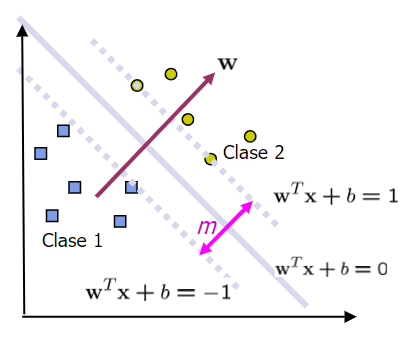
\includegraphics[scale  = 0.70]{Imagenes/maxim.png}
	\caption{Margen m maximizado}{Fuente: Adaptado de ~\cite{betancourt}}
\end{figure}

Una Máquina de Soporte Vectorial (SVM) aprende la superficie de decisión de dos clases distintas de los puntos de entrada. Como un clasificador de una sola clase, la descripción dada por los datos de los vectores de soporte es capaz de formar una frontera de decisión alrededor del dominio de los datos de aprendizaje con muy poco o ningún conocimiento de los datos fuera de esta frontera \cite{betancourt}.